% !TEX root = ../TechProject.tex

\graphicspath{{Chapter2/}}

\chapter{Machine Learning used in Music Recommendation Systems}



\section{The need for music recommendation systems}
Spotify, SoundCloud, Apple Music and other streaming services gives one access to a library of tens of millions songs. Music Recommendation systems are excellent at fitting a users preference whilst incorporating some level of filtering of an overwhelming amount of songs \citep{bollen_understanding_2010}. 

Music recommendation systems study users habits and taste, and with that information give out suitable recommendations. This aids the listener to discover new songs or artists they otherwise would not have found.

With this potential, a well made recommendation system could be a make or break for choosing one stream service from another. For this reason a lot of research gets poured into recommendation systems as an attempt to retain engagement and allow for company growth. 

 With recommending music, a lot of sub conscious factors come into play on what a user wants to listen to at a given time. This can range from characteristics and mood of the listener \citep{ferwerda_personality_nodate}  \citep{rentfrow_re_2003}, to what they get up to in day-to-day life \citep{gillhofer_iron_2015} \citep{wang_context-aware_2012}.  The users environment can have an affect as well \citep{kaminskas_location-aware_2013}. Observing a user made playlists also can reveal a lot on what groups of songs work for suited situations \citep{zheleva_statistical_2010} \citep{mcfee_hypergraph_2012}.
 
 A necessity for making a recommendation system suited for a type of product is taking into consideration the common place attributes of the product. Music lends itself to having a specific method due to short duration and high emotional connection. A recommendation system that uses these attributes to its advantage will be more successful than ones that don't.

\section{Collaborative Filtering}

Collaborative Filtering guesses users taste by looking at similar user-item connections. Using an explicit example, if a user rates something highly, it can provide similar suggestions from looking at other users ratings \citep{celma_recommendation_2010}.

The first known use of collaborative filtering is with Goldberg's Tapestry system, a mailing list filter where users collectively decide which type of emails get the most importance \citep{goldberg_using_1992}. The first instance of collaborative filtering being used was with a system called \textit{Ringo} where users would enter in music they rated and would get recommendation's pulled from similar users \citep{shardanand_social_1995}

\begin{figure}
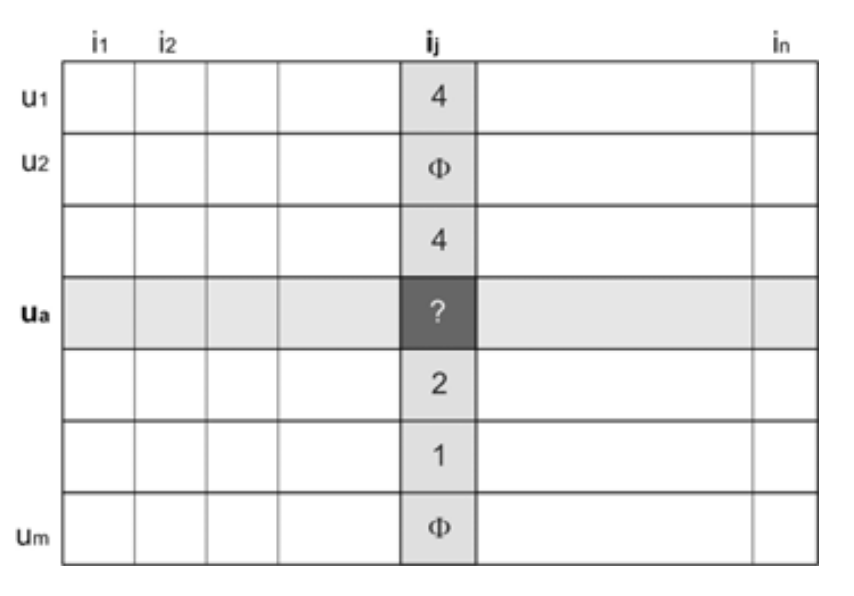
\includegraphics[scale=0.65]{images/collaborative_filtering}
\centering
\end{figure}

\section{Content Based Filtering}

\section{Clustering}

\section{Convoluted Networks}


% note that \Blindocument has 5 numbered levels, despite setting secnumdepth above. I (and many style guides) would suggest using no more than 3 numbered levels (incl. the chapter), with the option of a fourth unnumbered level.